\documentclass[11pt]{article}
\usepackage{amsthm,amsmath,amsfonts,amssymb}
\usepackage[ruled,noline,noend]{algorithm2e}
\usepackage{enumerate}
\usepackage[margin=0.75in]{geometry}
\usepackage{graphicx}
\usepackage[]{hyperref}

% set table of contents level
\setcounter{tocdepth}{2}

% for list stuff
\usepackage{enumitem}

% For code examples
\usepackage{listings}
\lstdefinestyle{mystyle}{
    breakatwhitespace=false,         
    breaklines=true,                 
    keepspaces=true,                 
    numbers=left,                    
    showstringspaces=false,
    showtabs=false,                  
    tabsize=2
}
\lstset{style=mystyle}

% So we can show the page number and section in the header
% TODO I want it to just show "Design Patterns" or "Architectures"
\usepackage{fancyhdr}
\pagestyle{fancy}
\fancyhf{}
\renewcommand{\sectionmark}[1]{\markright{#1}}
\fancyhead[L]{\nouppercase{\rightmark}}
\fancyfoot[R]{\thepage}
\renewcommand{\headrulewidth}{0pt}

% Remove numbers from titles but keep incremementors
\usepackage{titlesec}
\titleformat{\section}{\normalfont\Large\bfseries}{}{0pt}{}
\titleformat{\subsection}{\normalfont\large\bfseries}{}{0pt}{}
\titleformat{\subsubsection}{\normalfont\bfseries}{}{0pt}{}

% for comparison 
\usepackage{multicol}
% \setlength{\columnsep}{1cm}

\newenvironment{summary}{
    \begin{itshape}
}{
\end{itshape}
}

\newenvironment{components}{
    \begin{description}
}{
    \end{description}
}

\newenvironment{nfps}{
    \subsubsection{Non-functional Properties}
    \begin{description}[noitemsep,style=multiline,leftmargin=4cm]
}{
    \end{description}
}

\newcommand{\comparison}[2]{
    \begin{multicols}{2} [ \subsubsection{Comparison} ]
        {\bf Advantages} \\ #1
        \vfill
        \columnbreak
        {\bf Disadvantages}\\ #2
        \vfill
    \end{multicols}
}

\newcommand{\pattern}[1]{\newpage\subsection{#1}}

\begin{document}

% Add a title page and table of contents
\tableofcontents

\section{Design Patterns}

\subsection{Types of advantages}
\begin{description}
    \item[Ease of use]: Creating a subclass based on the base class is easy
        to manage, it only requires the subclass to provide either a
        concrete implementation of an abstract method, or a more specific
        implementation of a method that is allowed by the base class.
    \item[open-closed principle]: the design philosophy is to be ``Open to
        Extension, Closed to Modification''.  Here the base class provides a
        framework code that can be extended through inheritance to allow
        instances of new-but-related classes with new fields and methods.
        This allows designers to be achieve new design requirements without
        having to change the code of the base class, or the algorithms and
        data structures which operate on instances of the base class.
    \item[reusability of the code]: Duplication of code is minimized through
        the use of base classes to establish a common pattern among
        subclasses. ``Inheritance'' means subclasses only need to write down
        overwritten methods for the base class to use.
    \item[flexibility]: Due to its reliance on
        inheritance to establish the behavior of subclasses, usually
        subclasses are restrained to inheriting from one base class at a
        time. As a result, any subclass is restrained to follow the general
        behavior established by its parent base class.
    \item[maintainability]: Reading the flow of code is
        difficult due to the disjoint nature of the code. Code within the
        base class only provides the steps that its subclasses will take,
        whereas subclasses only contain details for a step. In addition,
        additional functionality is difficult to implement due to the tight
        coupling between classes. Adding features to the base class
        requires the change to be applied to all related subclasses.
\end{description}



\pattern{Visitor}

\begin{summary}
The visitor design pattern provides a method of separating an algorithm on an
object and the object’s actual class implementation.  Since the pattern
separates the visitor (operations) from the object structure, it's very easy to
add new visitors as long as the structure remains unchanged.
\end{summary}

Allows you to: \begin{itemize}
    \item add methods to classes of different types without much altering to
        those class.
    \item define external classes that can extend other classes without majorly
        editing them
    \item create a separate visitor concrete class for each type of operation
        and to separate this operation implementation from the objects
        structure.
\end{itemize}

Used when: \begin{itemize}
    \item there are many distinct and unrelated operations
    \item Object structure is not likely to be changed but is very probable to
        have new operations which have to be added
\end{itemize}


\comparison{
    \begin{itemize}
        \item Follows open/close principle
        \item Allows new operations to be added without changing implementation
        \item A visitor can have state
    \end{itemize}
}{
    \begin{itemize}
        \item Does not fit for pattern 1 that updates arguments frequently.
        \item Some non-hierarchy behaviors should not be implemented via
            visitor pattern, since they will be applied to whole system.
    \end{itemize}
}

\begin{nfps}
\item[Maintainability] Center to visitor, increases maintainability
\item[Testability] Each sub class has its own method to debug
\item[Extensibility] Easy to write own method
\item[Reusability] No need to change structures to add new operations
\end{nfps}

\begin{center}
    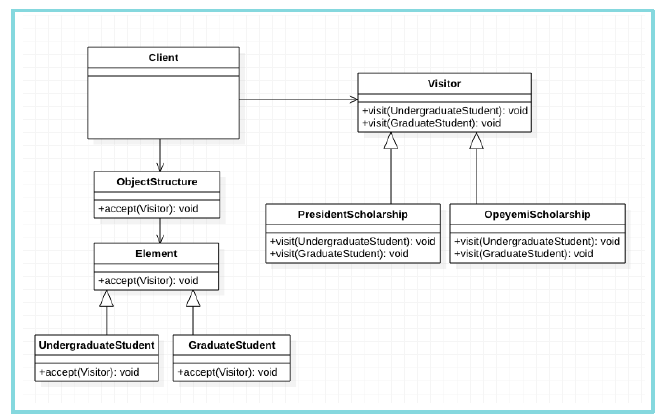
\includegraphics[width=0.5\textwidth]{./visitor}
\end{center}

\pattern{Template}
\begin{summary}
    Describes (and realizes) the common interactions between components. The
    {\bf template} pattern defines the skeleton of an algorithm for an
    operation while deferring some behaviour to the elements that are being
    operated on.
\end{summary}

Implementation details: \begin{itemize}
    \item Create a notion of an interface (either an interface or class) or
        a component of an algorithm that doesn’t vary between different
        datatypes (or both). Then use inheritance to create a specific
        implementation for the datatype addressed.
    \item in higher level languages (C\#, Java by type-erasure) where
        every class is a ``subclass'' of a super base class, (java.lang.Object
        in the case of Java), this can be used with many standard library
        algorithms and data structures
\end{itemize}

\comparison{\begin{itemize}
        \item ease of use: Creating a subclass based on the base class is easy
            to manage, it only requires the subclass to provide either a
            concrete implementation of an abstract method, or a more specific
            implementation of a method that is allowed by the base class.
        \item open-closed principle: The base class provides a
            framework that can be extended through inheritance to allow
            instances of new-but-related classes with new fields and methods.
            This allows designers to achieve new design requirements without
            having to change the code of the base class, or the algorithms and
            data structures which operate on instances of the base class.
        \item reusability: Code duplication is minimized through
            the use of base classes to establish a common pattern among
            subclasses. Subclasses only need to override methods that are not 
            defined for their use-case.
    \end{itemize}

}{\begin{itemize}
        \item flexibility: Due to its reliance on inheritance to establish the
            behavior of subclasses, usually subclasses are restricted to
            inheriting from one base class at a time. As a result, any subclass
            is restricted to follow the general behavior established by its
            parent base class.
        \item maintainability: Reading the flow of code is
            difficult due to the disjoint nature of the code. Code within the
            base class only provides the steps that its subclasses will take,
            whereas subclasses only contain details for a step. 
        \item tight coupling: Additional functionality is difficult to
            implement due to high coupling.  Adding features to the base class
            requires the change to be applied to all related subclasses.
    \end{itemize}
} % END of comparison

\begin{nfps}
\item[Something]
\end{nfps}

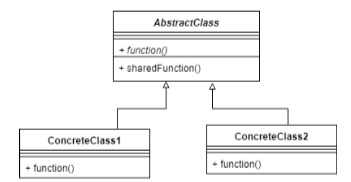
\includegraphics[width=0.5\textwidth]{./template1}
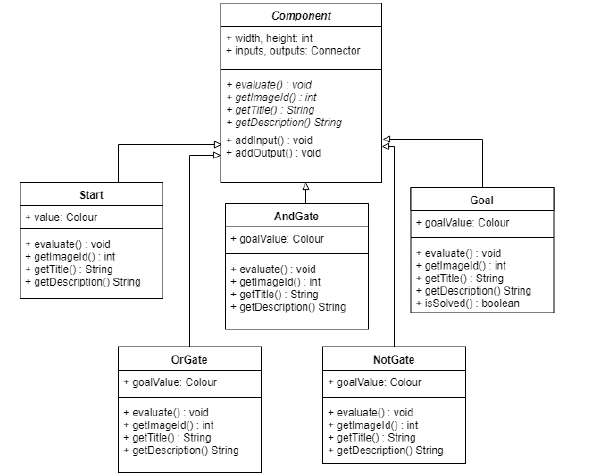
\includegraphics[width=0.5\textwidth]{./template2}

\pattern{Strategy}
\begin{summary}
    The {\bf Strategy} pattern resembles a {\bf State} pattern but it
    encapsulates algorithms instead of data. 
    
    % TODO what does this mean
    You can see that the Context class in the Strategy Class Model is an
    (aggregator) has a Strategy interface (aggregate).
\end{summary}

\comparison{\begin{itemize}
        \item Flexibility: a solution to a problem can use many options and it
            is easy to apply the selected algorithm. Users can choose the most
            suitable algorithm for their systems. 
        \item High encapsultation: it is easy to add, remove, or switch algorithms
            because each strategy is encapsulated into separate classes.
            Changing one algorithm does not affect the others. Additionally, 
            each algorithm can be tested independently.
        \item Loosely coupled: algorithms are not reliant on each other within the
            context entity. They can be changed or replaced without changing the
            context entity.
        \item Readability: the pattern reduces the number of conditional
            statements such as if-else statements or switch statements. Conditionals can
            be computationally expensive.
        \item Reusability: Algorithms and behaviours can be easily reused, due
            to their high level of encapuslation.
    \end{itemize}

}{\begin{itemize}
        \item Prior knowledge about each algorithm is required. Users must know
            about various strategies/algorithms to select the best one for
            them.
        \item Performance: It increases the number of objects in the application.
            a. It requires many objects to do its job, which increases memory requirements.
            b. It may cause an impact on performance of the application.

    \end{itemize}
} % END comparison

\begin{nfps}
\item[Maintainability] It is easy to modify or replace algorithms, which can be
    done in separate classes.
\item[Testability] Since each algorithm is encapsulated into separate classes,
    it allows developers test each algorithm separately. This is less complex
    and tends to be more reliable.
\item[Extensibility] When users need new algorithms, it is easy to add them
    since it can be done by creating new strategy classes. This creation
    process does not affect other algorithms.
\item[Reusability] Algorithms and behaviours can be easily reused because they
    are encapsulated.
\end{nfps}

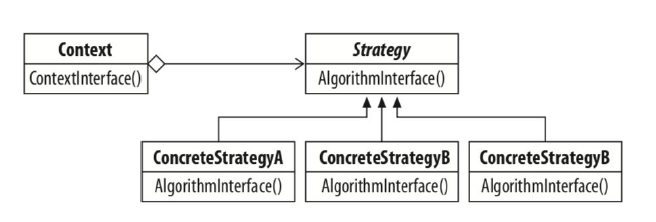
\includegraphics[width=0.5\textwidth]{./strategy}

\pattern{State}
\begin{summary}
    Given an object that needs to change its behaviour based on its
    internal state at run-time, the {\bf State} pattern encapsulates the number
    of states in a given context. A context calls its cooresponding
    state to perform specific behaviour, which changes based on the
    current value of the state object.

    This pattern should be used when the application's behaviours can be
    clearly divided into independent states that have specific and distinct
    behaviours, and when the application needs to be able to change its state
    and behaviours at run-time.

    Example. A flashlight has two states, on and off. When the flashlight is on,
    pressing the power button will turn off the flashlight, and vice versa.
\end{summary}

Implementation details: \begin{itemize}
    \item {\sc Context}: an instance of a class that owns (contains) the state.
        The context is an object that represents a class that can have more
        than one state.
    \item {\sc State}: an abstract class or interface. {\sc State} is the base
        class for all possible states. It defines all possible method
        signatures that all states must implement.
    \item {\sc ConcreteState}: a class that implements the actual state
        behavior for the context object. It inherits from the base {\sc State}
        class. The {\sc ConcreteState} class must implement all methods from
        the abstract base class {\sc State}.
\end{itemize}

The State design pattern allows full encapsulation of an unlimited number of
states of a context. The context object calls its state object to perform
specific behavior. The behavior is differentiated by the concrete state at the
run-time.

\comparison{\begin{itemize}
        \item Maintainability: Adding, removing, and modifying states is
            streamlined and simple via modifying the corresponding concrete
            state object.
        \item Readability: Improved cohesion due to aggregation of all
            behaviours of a given state in its corresponding concrete state
            class.
        \item Low coupling: Each state is independent of each other states'
            behaviour and modifications
    \end{itemize}

}{\begin{itemize}
        \item Maintainability: Since each concrete state is implemented as a
            class, more classes are required and more code needs to be written
        \item Maintainability: must implement all the functions in the abstract
            state, even if a given class is not related to a function used
            primarily in a different class.
        \item Maintainability: Difficult to maintain due to all states being
            required to implement a new function when new functionality is
            added to the interface. 
    \end{itemize}
} %END comparison

\begin{nfps}
\item[Scalability]: The State design pattern allows an unlimited number of
    states for a given object.
\item[Adaptability]: Adding, removing, and modifying states is as simple as
    modifying a concrete object class.
\item[Dependability]: Since each state is independent of the others, states
    with errors do not interfere with the functionality of other states.
\item[Negative Maintainability]: Since each state requires a separate class,
    there can be a large number of concrete classes, resulting in the code base
    being harder to maintain. In addition, since every method in the abstract
    class must be implemented in the concrete classes, much more code needs to
    be written.
\end{nfps}

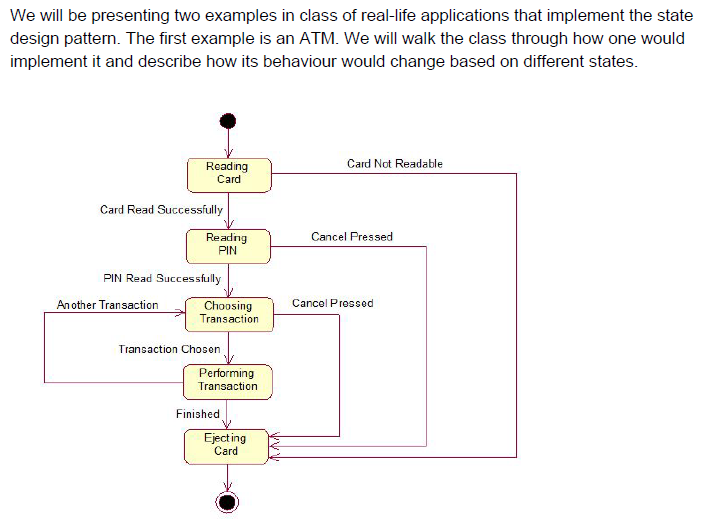
\includegraphics[width=0.5\textwidth]{./state1}
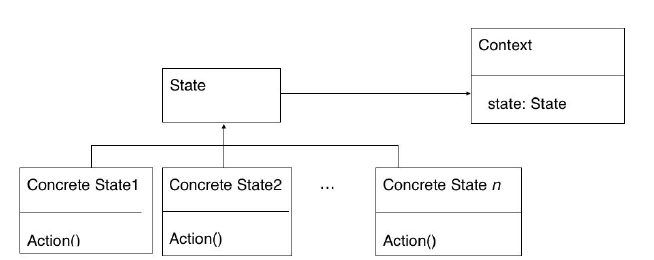
\includegraphics[width=0.5\textwidth]{./state2}


\pattern{Proxy}
\begin{summary}
    A {\bf proxy} is a wrapper or agent object that is being called by the
    client or user to access the real object behind the scenes.

    This pattern is widely used in applications that require security
    protection and access control.
\end{summary}

\subsubsection{Implementation details}
In general, a proxy is a class that is functioning as an interface (or
placeholder) to something else. 
\begin{description}
    \item[Virtual Proxy (a type of caching)] Proxy returns a default or cached
        result if the real object either takes some time to create or involves
        heavy computation. Virtual proxies delay the initialization or 
        computation of the real object until it is needed.
    \item[Remote Proxy] Used when a resource is remote. Communicating with the
        real object might involve serialization or marshalling of data. That
        logic is encapsulated in these proxies. 
    \item[Protection Proxy] Used for access control and partial encapsulation.
        Users will only have access to functions provided by the interface. 
        The application provides different interfaces to different clients with
        different access rights.
\end{description}

\comparison{\begin{itemize}
        \item Maintainability: Internal change to the ``Real Subject'' does
            not affect the proxy consumers because access is abstracted through 
            the proxy interface.  Developers can easily add new methods into
            the interface for clients to use.
        \item Low Coupling: reduces the coupling between client and the real
            subject by providing an abstracted interface between the client
            and subject.
        \item Performance: The use of caching in the proxy can increase
            the performance of some systems.
    \end{itemize}
}{\begin{itemize}
        \item Performance: The extra layer of abstraction could impact 
            performance in some cases.
    \end{itemize}
}% END comparison

\begin{nfps}
\item[Security] Proxy pattern guarantees that only authorized users can access
    the resource. Different interfaces can be seen as different access rights.
\item[Performance] The initialization of expensive objects can be delayed by
    using a proxy object that exposes the same interface as the original 
    object. Caching and delayed initialization allow for performance gains.
\item[Negative Inconsistency] ``This pattern introduces another layer of
    abstraction which sometimes may be an issue if the {\sc RealSubject} code
    is accessed by some of the clients directly and some of them might access
    the {\sc Proxy} classes. This might cause disparate behaviour.'' 
\item[Negative Ambiguity] The client may not know that the {\sc RealSubject} it
    is accessing now is not same as the previous one.
\end{nfps}

\subsubsection{Example}
Proxies are often used to interface with a network connection, a large object
in memory, a file, or some other resource that involves heavy computation or
that is impossible to duplicate.

The banking application below with deposit functions is an example.

\begin{center}
    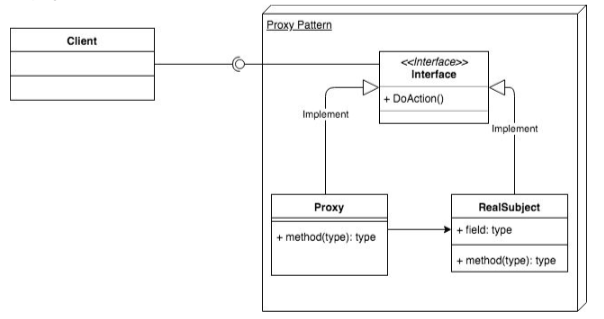
\includegraphics[width=0.4\textwidth]{./proxy1}
    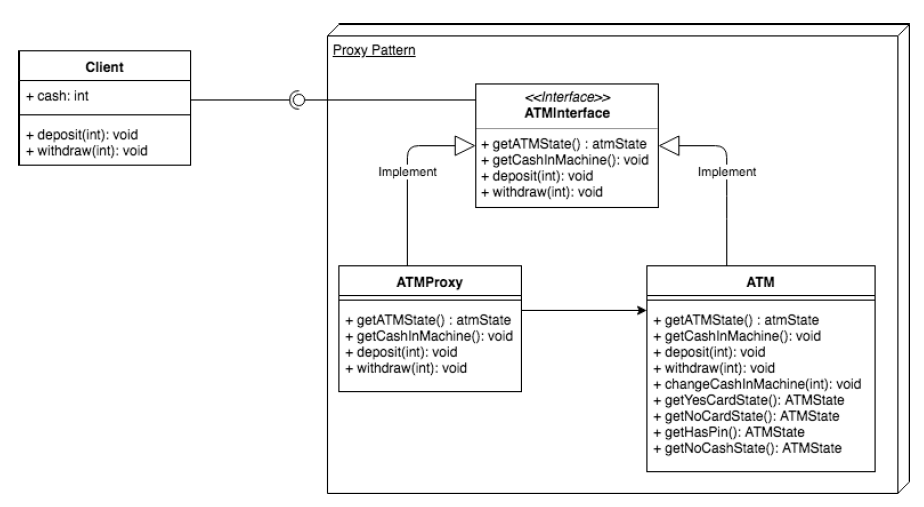
\includegraphics[width=0.4\textwidth]{./proxy2}
\end{center}


\pattern{Observer}
\begin{summary}
    The {\bf Observer} pattern is characterized by a subject and many observers
    which are ``observing'' the subject and reacting to change. The subject
    keeps a list of objects to notify when it changes, but otherwise has
    no information on the observer objects (other than the notify interface).
\end{summary}

\comparison{\begin{itemize}
        \item Loosely Coupled: Since a subject only knows about a observer
            interface and not specifically what each concrete observer does. 
            One can modify the object and subject independently, so long
            as they maintain the observer interface.
        \item One to Many Relationship: When a subject changes state (or data),
            all its dependent observers are notified and updated automatically.
            When the system needs to send data to many objects on change, it
            can be an efficient solution. 
        \item Consistency: As the observers are updated automatically
            when the subject changes its state, they are consistent with the 
            subject.
\end{itemize}
}{\begin{itemize}
        \item Inefficiency: When each observer is also a subject, and each
            subject has a large amount of observers, the speed of processing
            the notification to a target object is slow (this is usually
            implemented as a for loop). This is because there are a lot of
            repeated ``notifies''. Some of the observers in the observer list
            have already been notified but there is no accurate way to detemine
            if it has been notified or not.
        \item Circular dependency: cyclical recursive calls can occur when
            there is an observer loop, which may lead to operating system
            panic. A circular dependency occurs when the UML has a cycle and
            each dependency has a notify function. This is easy to detect, but
            in practise if the design is complex then it may require more
            effort to solve. The problem is worse for highly automated system.
\end{itemize}
}%END comparison

\begin{nfps}
\item[Scalability] Using the observer pattern makes scaling an application
    easy, since adding more observers to a subject is trivial. In the MVC
    design pattern, a {\sc Model} can have any number of {\sc Views} observing
    it, and each {\sc View} will take the data relevant to it from the {\sc
        Model} to display.
\item[Maintainability] It is easy to maintain and organize an observer system. 
    Removing and adding observers is simple, and since observers are completely
    decoupled from the subject the overall system is flexible and can be
    changed to meet the needs of developers.
\item[Negative Inefficiency] Inefficiency occurs when there
    is a long chain of dependency or objects are in several other subjects’
    observer lists. The number of calls can grow exponentially if there
    are repeated objects in the notify list. The Observer pattern should be
    avoided if there would be a long chain of dependencies between observers.
\end{nfps}

\begin{center}
    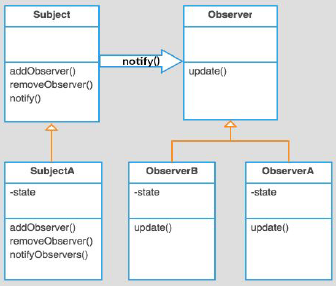
\includegraphics[width=0.4\textwidth]{./observer1}
\end{center}


\pattern{Mediator} 
\begin{summary} 
    A {\bf mediator} is an object that encapsulates a web of relations or
    interactions between sets of other objects, acting as an intermediary which
    decouples dependent objects. This allows objects to communicate without
    referring to each other explicitly. Instead, objects send requests to the
    mediator, which processes and directs them to the appropriate subject. 

    Mediator patterns are best suited for situations where a set of objects
    communicate in complex ways. Multiple unstructured interdependencies
    creates difficulty in understanding the process of events and the ability
    to reuse objects.
\end{summary}

\comparison{\begin{itemize}
        \item Low coupling: Since objects communicate with a mediator instead
            of directly, they are unaware of other component's implementations. 
        \item Maintainability: adding, deleting, and modifying components and
            relations is easy since components are encapsulated. By separating
            relations between classes and grouping them in a different class,
            any change to one component will not affect the rest of the code.
        \item Code reuse: Since objects communicate in a common shared way
            with a central mediating object, code can be reused between
            objects. 
        \item Flexibility: Mediators model the inter-relationships of
            objects to allow modification and extension of these
            inter-relationships through subclassing and allows flexibility.
        \item Readability: Centralized communication between objects can make
            it clearer when objects are communicating, and with which other
            objects. 
\end{itemize}

}{\begin{itemize}
        \item Readability: The mediator can become ``God object'' that knows
            too much or does too much. This can lead to a complicated and hard
            to understand system.
        \item Maintainability: The system can become counterproductive, 
            ineffective, and risky if the mediator controls too much, or if
            objects communicate in a complex and poorly defined way.
\end{itemize}
}% END comparison

\begin{nfps}
\item[Complexity] It increases developer understanding needed to work with
    the components. Individual components have clearer interactions, which are
    defined through a standard interface. The {\sc Mediator} class that
    centralizes communication creates an easy way to see all relations.
\item[Scalability] Low coupling due to the lack of dependencies between
    components allows for new components/relations which will not affect
    existing components/relations. The addition of components from other
    applications just requires a new mediator. 
\end{nfps}

\subsubsection{Example}
When texting your friend, you are not making a direct connection between your
phones. Many mediators are involved in this process. Bits that make up your
message is sent to a cell tower closest to you. The switching service is then
handled by your carrier which helps establish the connection to your friend on
your behalf. The message is then passed to the cell tower closest to your
friend. Finally, the message appears on your friend’s phone. In this scenario,
your carrier is the main mediator.

\begin{center}
    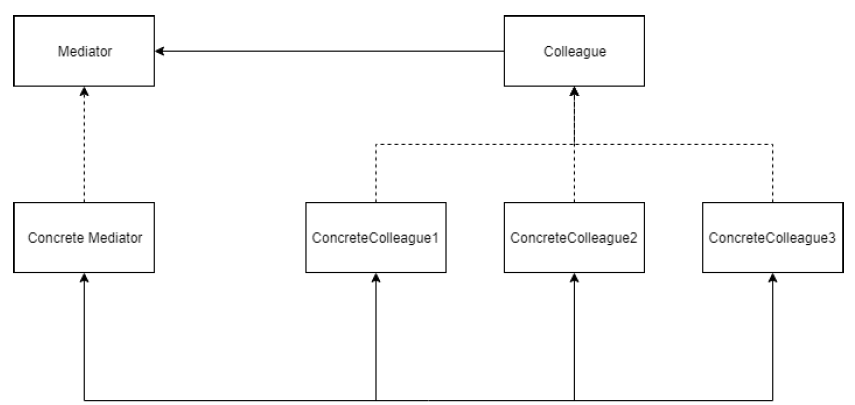
\includegraphics[width=0.4\textwidth]{./mediator1}
    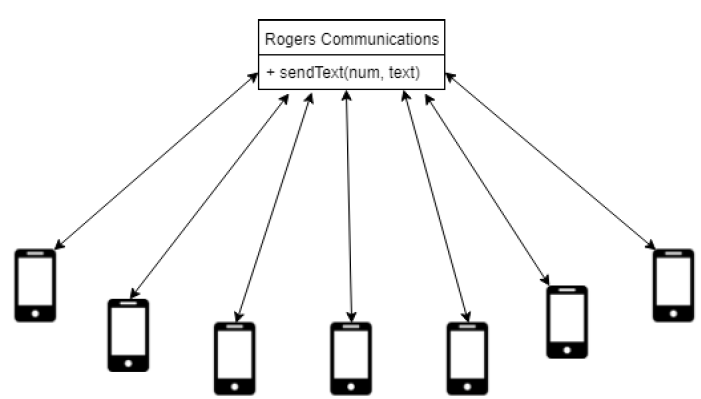
\includegraphics[width=0.4\textwidth]{./mediator2}
    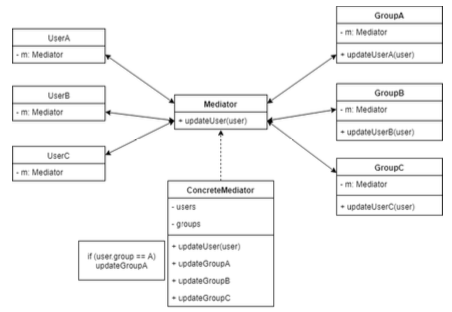
\includegraphics[width=0.4\textwidth]{./mediator3}
\end{center}

\pattern{Flyweight}
\begin{summary}
An object that minimizes memory usage by sharing as much data as possible with
other similar objects.

A way to use objects in large numbers when a simple repeated representation
would use an unacceptable amount of memory. While often some parts of the
object state can be shared. The {\bf Flyweight} pattern describes how to share
objects to allow their use at fine granularity without prohibitive cost. 

Flyweights should be used when a component requires a large number of objects,
the storage costs are high for the number of objects needed, it would be
difficult to maintain the number of objects, and the application does not
depend on object identity.
\end{summary}

\subsubsection{Implementation}
Each ``flyweight'' object is divided into two pieces: the state-dependent
(extrinsic) part, and the state-independent (intrinsic) part. Intrinsic state
is stored (shared) in the Flyweight object. Extrinsic state is stored or
computed by client objects, and passed to the Flyweight when its operations are
invoked. Flyweights are stored in a Factory's repository. The client restrains
herself from creating Flyweights directly, and requests them from the Factory.
Each Flyweight cannot stand on its own. Any attributes that would make sharing
impossible must be supplied by the client whenever a request is made of the
Flyweight.

\comparison{\begin{itemize}
    \item Save memory by reduce the repeat data
    \item Reduction of number of objects to handle when application requires a large number of objects
    \item If the objects are naturally immutable, then impact on performance of using a Flyweight is negligible
    \item Working with Flyweights is easy in a language like Java where all object variables are references and a garbage collector is responsible for removing old objects.
    \end{itemize}
}{\begin{itemize}
    \item Move state outside the object breaks encapsulation
    \item If the object is not naturally immutable, then might affect performance in some case
    \item Little trickier in language like C++ where objects can be allocated as local variables on the stack and destroyed as a result of programmer action.
    \end{itemize}
} %END comparisson

\begin{nfps}
\item[Data integrity] might lose if the data is not intending to share (lost encapsulation)
\item[Performance] might increase in some case like browsing the website with same image, save download same image time. However, in some case the performance might decrease due to save memory that require search the data.
\item[Reusability] since flyweight save common use the same data in just one copy, in that case save certain memory. It is similar to the helper function, that the same data can be used in different class.
\end{nfps}

\begin{center}
    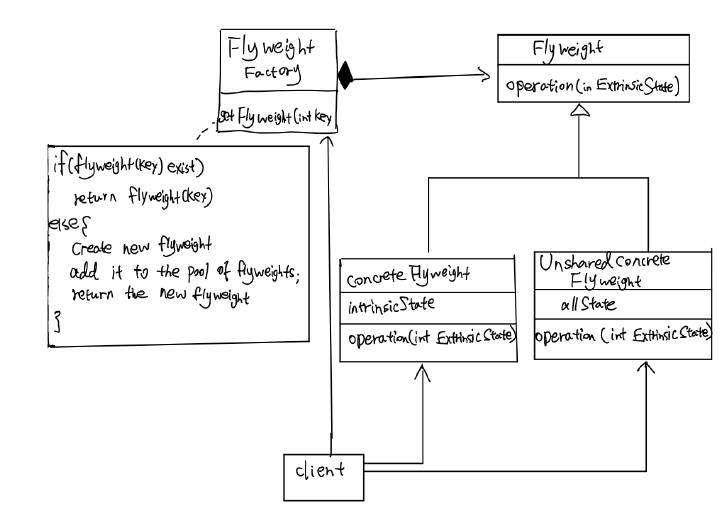
\includegraphics[width=0.4\textwidth]{./flyweight}
\end{center}

\pattern{Factory}
\begin{summary}
    The {\bf Factory} method pattern is a class-creation design pattern,
    meaning that its purpose is to deal with object creation.

    The factory method pattern creates a predefined interface for object
    creation within a parent class, while at the same time allowing for
    child classes to determine exactly what type of objects are created. This
    makes it so that object creation responsibility falls on the child classes,
    and the class that uses the new object can treat the process of object
    creation as a black-box. The class only needs to be concerned with
    providing the correct data and it can assume that the correct object will
    be instantiated and returned to them.

    This pattern proves to be very useful over time as it can significantly
    reduce maintenance costs.
\end{summary}

\subsubsection{Implementation}
The Factory pattern standarizes object creation through the use of inheritance
and subclasses to instantiate objects. It uses a ``factory method'' to create
objects, rather than the developer using the constructor of the objects
themselves. This allows for greater flexibility and dynamism when determining
what type of object to construct. This factory method is specified within an
interface in a parent class, whose behaviour is then implemented by child
classes. These child classes are then responsible for the actual instantiation
of the object, and can specify the type of the object. This pattern allows for
many different child classes that can all implement the factory method and
return different types.

\comparison{\begin{itemize}
        \item Readability: It provides a level of abstraction for object
            creation. Instead of a developer needing to fully understand
            what subclass they need and how to instantiate it, they can use the
            factory’s exposed method to generate an instance. 
            
        \item Low coupling: Allows for a separation of concerns between an
            object’s creation and usage. There is a level of abstraction that
            means the object instantiated can be determined at runtime. 
            The developer can request an object that will meet the abstract
            product’s requirements without knowing what subclass will be 
            created.

        \item Encapsulation: This pattern can help developers hide the
            implementation details of the subclass by only exposing an
            interface to the user. This leads to a decrease in coupling within
            the overall application. 
        \item Maintainability: The factory method pattern also improves
            the maintainability of the system. Developers only need to create a
            new subclass which implements the exposed common interface in order
            to create a new type without bother implementing the entire
            structure of the new class type.
    \end{itemize}

}{\begin{itemize}
        \item Efficiency: If it is not used within the correct scenarios. The
            additional layer of overhead that the pattern adds by requiring the
            creation of subclasses that are tasked with object creation can 
            become inefficient. With simple, low complexity classes that do not
            change, it is much easier to just instantiate objects within the
            parent class rather than delegate that works to child classes.

        \item Maintainability: If the pattern is overused to allow for dynamism
            within a system that does not need it, it will become overly
            complex. If every object is created through a factory method (thus
            creating new base classes, base products, and each concrete
            implementation) the code will be unnecessarily complex, difficult
            to follow, and hard to test. Thus this design pattern should only
            be used when its benefits clearly outweighs the added overhead.
    \end{itemize}
}% END comparison

\begin{nfps}
\item[Evolvability] All that is required to meet new requirements is to create
    another subclass of the object with the new functionality.
\item[Complexity] Components can be created and perceived as their parent
    class. The developer only has to work with the abstraction and not the
    specifics, thus decreasing the overall complexity of the system.
\item[Negative Efficiency] The added overhead of creating child
    classes can be quite expensive.
\item[Negative Complexity] The additional abstraction through the factory can
    negate any complexity benefits, and even make the code base more complex
    and difficult to understand.
\end{nfps}

\begin{center}
    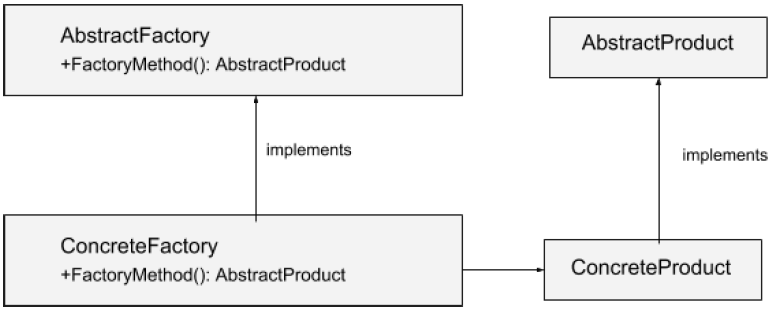
\includegraphics[width=0.8\textwidth]{./factory}
\end{center}

\pattern{Facade}
\begin{summary}
    The goal of a {\bf Facade} is to create an object that provides a simplified,
    unified interface to a more complex, larger body of code such as the
    various interfaces of a subsystem. 
\end{summary}

\comparison{\begin{itemize}
        \item Low Coupling: Clients are decoupled from a subsystem. Avoid tight
            coupling between a client and it’s subsystem by introducing an
            independent facade interface
        \item Readability: Simplify complex code blocks and provide convenient
            methods. Wrap several code blocks to a more elegant set of APIs.
        \item Maintainability: Facade provides a single point of entry to a
            subsystem, improving usability and simplicity.
\end{itemize}

}{\begin{itemize}
        \item Efficiency: Adds a layer to the code stack, which may affect
            performance.
        \item Readability: Developers still need to know implementation
            details, and the pattern will increase the size of the code base.
        \item Evolvability/Adaptability: if the Facade is the only access point
            for the subsystem, it will limit the features and flexibility that
            ``power users'' may need.
\end{itemize}
}% END comparison

\begin{nfps}
\item[Complexity] The pattern allows the client to work through this singular
interface to existing subsystem components. 
\item[Evolvability] Working through a Facade minimizes dependencies for the
client, making it easier to implement, change, and use.
\end{nfps}

\subsubsection{Example}
Facade is an extremely versatile pattern, able to be applied to various
situations. This can include:\begin{itemize}
\item Database access
\item Network communication
\item Any code libraries
\item Input/output interfaces
\end{itemize}

Real life example is the customer service department at any company. The
company handles many things such as sales, returns, order inquiries and
shipping. It would be very annoying if you had to access any of these
departments through different means, however the use of a customer service
department acts as a facade and simplifies the process.

\begin{center}
    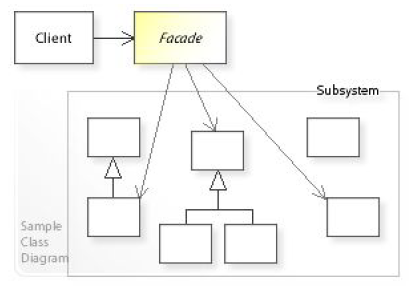
\includegraphics[width=0.8\textwidth]{./facade}
\end{center}

\pattern{Decorator}
\begin{summary}
    Decorator pattern allows functionalities to be added or removed from an
    existing object, either statically or dynamically, without changing its
    original structure. Also, in these processes, the behavior of other objects
    from the same class will not be influenced. It resolves the problem when
    subclassing would result a large number of subclasses. It is also known
    as ``Wrapper'' Pattern because this pattern utilized a ``wrapper'' (decorator class)
    that wraps the original object and appends more functionalities while leaving
    class methods signature unchanged.
\end{summary}

\subsubsection{Implementation}
Composite and Decorator have similar structure diagrams since they both rely on
recursive composition to organize a number of objects. Comparing with composite
pattern, the decorator pattern can be viewed as a degenerate composite with
only one component. However, a decorator adds additional responsibilities.

Component: It is an interface implemented by both, concrete component and
decorators. It is also the interface for objects that can have functionalities
added to them dynamically.

Concrete Component: Normally, it is known as a base which needs to be
decorated. It also defines an object to which additional functionalities can be
added or removed.

Decorator: It represents a base class for all decorators. It maintains a
reference to a component object and defines an interface that conforms to
component interface.

Concrete Decorator (ie. Co ncreteDecA, ConcreteDecB): It extends the
functionality of the component by adding state or adding behavior.

\comparison{\begin{itemize}
        \item Decorator Pattern is flexible and easy to extend functionalities.
        \item Decorator Pattern is a good solution to permutation issues
            because a concrete pattern can be wrapped with any number of
            decorators.
        \item Decorators allow behavior modification at runtime rather than
            going back into existing code and making changes.
        \item It is easy to debug each functionality seperately.

    \end{itemize}

}{\begin{itemize}
        \item Since there are many decorators warp around the component, it is
            hard to have decorators keep track of other decorators.
        \item It can be complicated to initialize a concrete component wrapped
            with many decorators. Sometimes, we may miss some of them.
        \item Abstract decorator must provide common interface.
    \end{itemize}
}%END comparison

\begin{nfps}
\item[Complexity] The pattern is extremely reusable by adding new object types
    in the decorator section to fit in what system requires and needs. New object
    types can be built on objects that already exist. It is easy for them to
    decorate these objects because decorator pattern is efficient and flexible.
\end{nfps}

\begin{center}
    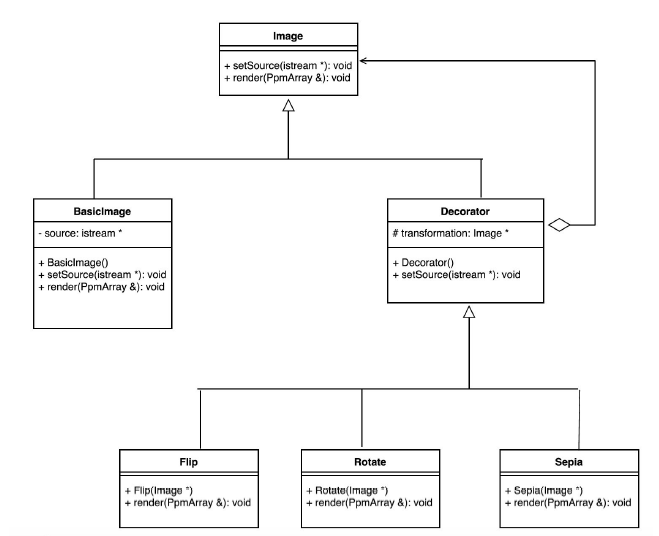
\includegraphics[width=0.8\textwidth]{./decorator}
\end{center}

\pattern{Composite}
\begin{summary}
Used to manage a hierarchy of components, each of which could be a composite,
or a leaf. Components use a single interface, which allows the user to call
methods without having to know which type of component it is. Every component
can be treated as its own entity thus allowing the whole system to be broken
down into parts.  

The main theme of the {\bf Composite} pattern is ``Containers that contain elements,
each of which could also be a container''

The composite design pattern should be applied when multiple objects are being
used in the same way in which each object has nearly identical code.
Additionally if the client does not care about the type of object it interacts
with than the composite design pattern is a good choice as it allows the client
to operate on objects without the concern for type.
\end{summary}

\subsubsection{Vocabulary}
\begin{description}[noitemsep]
\item[Client] Only aware of Leafs/Composites through the Component Interface
\item[Component] An item in the composite pattern, that can either be a leaf or a composite
\item[Leaf] Primitive component that cannot contain other components
\item[Composite] Component than can contain other components
\item[Topology] The composite pattern is most often used to represent
hierarchies and tree structures. Composites contained in another composite
represent a subsystem and are functional without knowledge of its parent.
\end{description}


\comparison{\begin{itemize}
\item Readability: The composite pattern simplifies client code that interacts
with complex tree structures, since the user does not have to know if they are
dealing with a leaf or a composite.
\item Evolvability: Makes it easier to add new kinds of components. New
components will work with existing client code without client needing to
change.
\end{itemize}

}{\begin{itemize}
\item Adaptability: all classes in the hierarchy follow a similar interface,
    which can lead to an overly general design. Therefore it is more difficult
    to restrict the components of a composite. Since all the classes implement
    an abstract interface this is not possible without a run-time check for the
    desired components.
\item Evolvability: the composite pattern will increase change resilience
    for adding specific properties or restrictions to components, since
    different types of components are often treated uniformly.
\end{itemize}
} %END comparison

\begin{nfps}
\item[Adaptability] The composite design pattern forces containers to work with
    child nodes through a common interface which allows for recursive
    operations on the entire hierarchy. This means that as new compositions and
    leaves are added to the hierarchy they can adapt to the existing code.
\item[Low Complexity] All classes follow a similar interface so the client
    does not have to worry about class specific code. The client can just treat
    primitives and composites as homogenous classes.
\item[Low Coupling] The composite design pattern reduces coupling by utilizing
    the same interface for each of the components. Whether it is a leaf or a
    composite, the class does not need to know any information about the other
    classes. 
\end{nfps}

\subsubsection{Example}
Using the composite pattern in this example lets the user interact with the
entire hierarchy easily, lets them break the tree into subtrees, and allows
users to add new type of components if it is necessary in the future.
Note that {\sc Folder} implements {\sc add()} and {\sc remove()} which are not
declared in the interface. There are cases where both types of components must
have the exact same interface, thus occasionally these functions are declared
in the component, but would cause an error if the user tries to add to a leaf.

\begin{center}
    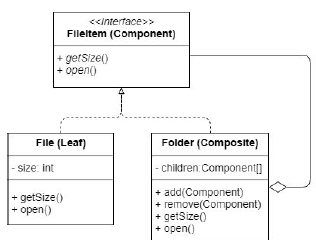
\includegraphics[width=0.4\textwidth]{./composite1}
    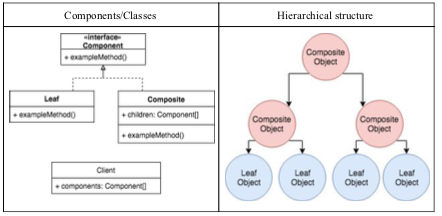
\includegraphics[width=0.5\textwidth]{./composite2}
\end{center}

\pattern{Command}
\begin{summary}
    The {\bf command} design pattern is a behavioral design pattern that is
    used for objects to issue requests/commands to receiver objects, while
    maintaining modular design. 
    
    It does this by encapsulating a command as an object type, thus allowing
    multiple operations of varying complexity that can be performed on a
    receiver. 

    It seeks to solve the problem of supporting potentially thousands of
    commands, for many different receiver objects, without hard-coding in
    commands to specific receivers. 
\end{summary}

\subsubsection{Use-case}

Hard-coding actions is very space inefficient because you will need to support
two different classes to perform the same operation if, for example, you are
turning both a radio and a TV on. 

The command pattern solves this by decoupling the command caller (the invoker)
from the object that knows how to perform the request. Thus, the invoker has no
knowledge of who will perform a given task. In the TV example, there would be 1
command called {\sc turnOn} which can be called on both TV and Radio types
depending on what receiver is in the concrete command.

Concrete commands consist of receiver object interface to perform actions
on different receiver objects.

\comparison{\begin{itemize}
        \item Complexity: The client could be oblivious to the implementation. 
            It does not care about the related problems of the task such as
            user-server synchronization and security, and it also has no idea
            about the actual business process. 
        \item Evolvability: The structure can be easily extended, due to each
            command is an independent class.
        \item Complexity: the history stack feature helps the invoker to trace
            back previous commands, and execute undo operations.
        \item Low coupling: the invoker has no knowledge of who will perform a
            task, allowing for loose coupling, and making it easier to add new
            commands without modifying existing code.
    \end{itemize}
}{\begin{itemize}
        \item Efficiency: will be very bulky if the client knows the business
            process very well, or the process is very simple. This will be a
            major restriction of a real-time system. 
        \item Complexity: because each command is a separate class, the
            extension of the system will make the code management difficult.
        \item Complexity: Each command fulfills an interface of a class, thus
            every subclass has to implement all of the interfaces that relate
            to. This also generates a lot of redundant code.
    \end{itemize}
}% END comparison

\begin{nfps}
\item[Extensibility] Command Design Pattern is perfect for
    achieving loose Coupling and high Cohesion. Invoker has a Command Interface
    not the concrete commands, which means invoker is loosely coupled with the
    concrete commands. New Concrete commands can be easily created under
    interface and invoker, with no need to know about the new concrete
    commands.  When new receivers are added, invokers don't need to know all
    the details.  Invoker just needs command interface for calling the concrete
    commands.

\item[Maintainability] The Command Pattern has high cohesion this means that
    classes now have well-defined, narrow responsibilities. Each concrete
    command class focuses on specific action on the receiver. It is much easier
    to maintain as these classes are less frequently changed. Each concrete
    command consists of receiver interface, which can be used to perform
    specific action on the receiver object.

\item[Scalability] Different receivers and commands can be added, which means
    more functionality can be added without affecting original workflow. When
    new receiver objects are created, new concrete commands are created which
    do not affect old concrete commands. As a result, original functionality is
    not affected. Applications using command design pattern have an advantage
    of high scalability, where new objects are created to achieve new
    functionality.

\end{nfps}

\begin{center}
    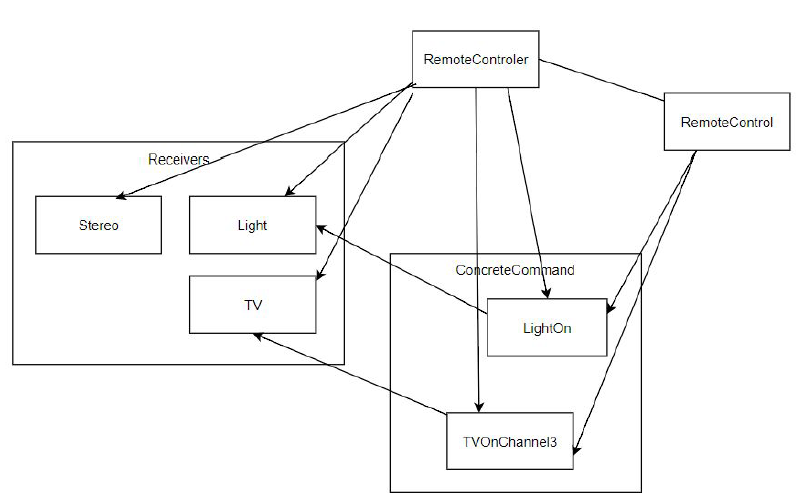
\includegraphics[width=0.4\textwidth]{./command}
    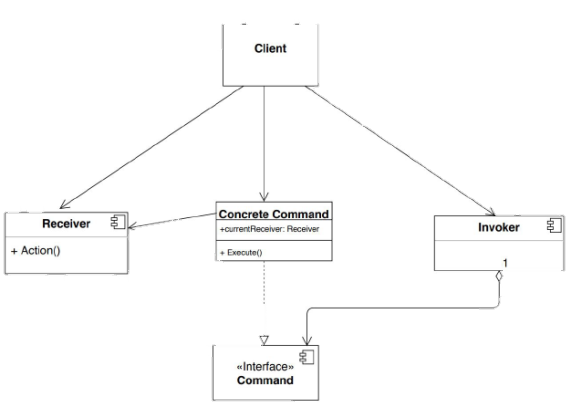
\includegraphics[width=0.4\textwidth]{./command2}
\end{center}


\newpage
\section{Architexture Styles}


\pattern{Virtual Machine (VM)}
\begin{summary}
    Static description: The {\bf virtual machine} is a middleware between the
    user and physical machine.

    Dynamic description: The {\bf virtual machine} style allows separation
    between user applications with Operating systems. This allows scalability
    and decouples layers so developers can ignore hardware issues.
\end{summary}

\subsubsection{Functional Properties}
\begin{description}
    \item[Multiple Operating Systems] Using a virtual machine
        allows a user to install and use multiple operating system on one
        physical machine. This reduces costs, as users no longer need to
        purchase additional physical machines to run separate operating systems
        and software. This also increases productivity and efficiency since all
        tasks can be performed on a single machine instead of on multiple
        machines.

    \item[Resource Sharing] There is a layer of software between the virtual
        machine and the host called the {\bf hypervisor} that is responsible
        for dynamically allocating resources from the host's memory to the
        virtual machine to allow multiple virtual machines to share
        resources between themselves. This allows a user to transfer files
        between virtual machines and the host (for example, to compile for
        different systems) without the hassle of needing to transfer files
        between machines.
\end{description}

\begin{nfps}
\item[Scalability] Without the need to purchase vast amounts of physical
    hardware to support different OS's, setting up virtual machines is much
    cheaper and less time consuming. New virtual machines can be added or
    expanded upon without having to add additional physical resources.

\item[Maintainability] Due to the nature of virtual machines being pieces of
    software, backups of virtual machines can be made easily as the states of
    these machines can be easily recorded into files. Since the states of
    virtual machines are just files on the host, they can also be easily cloned
    and used on another physical machine.

\item[Security isolation] Virtual machines are designed in such a way to make
    software think it is running in a native operating system on a physical
    machine and that includes viruses and malware. Malware will only run on the
    virtual machines which will have no impact on the host. Since
    backups are easily made, a clean version of the virtual machine can also be
    easily restored.

\item[Negative Efficiency] Virtual machines are often slower than physical
    machine due to indirect access to the host hardware. This means there is
    higher response time.

\item[Negative Efficiency] Virtual machines use more resource due to
    program overheads. For example, some virtual machines allocate disk space
    but it's idle. This lends to waste in disk/memory space since the host
    machine thinks it is in use.

\item[Negative Dependability] When running multiple virtual machines on the
    host OS there could be conflicts which lead to crashes and faults.
\end{nfps}

\begin{center}
    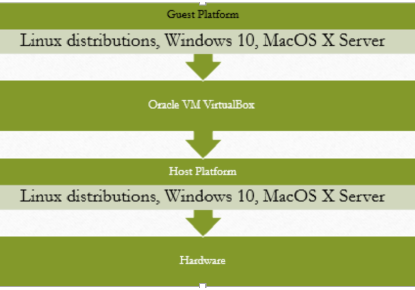
\includegraphics[width=0.4\textwidth]{./virtual-machine}
    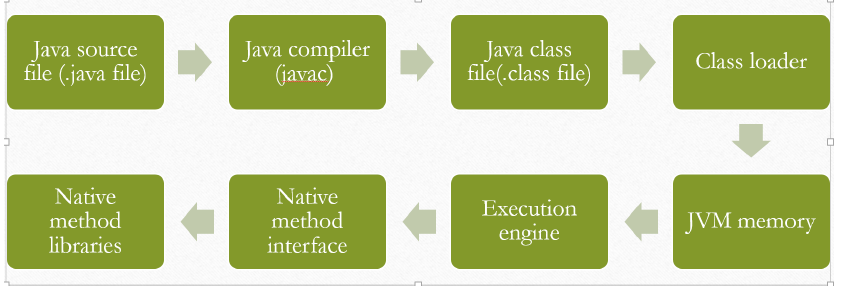
\includegraphics[width=0.4\textwidth]{./virtual-machine2}
\end{center}

\pattern{Publish and Subscribe}
\begin{summary}
    Allows publishers (senders) to broadcast messages to several subscribers
    (receivers) without them being tightly coupled. Essentially, the publishers
    are unaware of which application is going to receive the message whereas
    the subscribers do not really care about who actually sent it.
\end{summary}


\subsubsection{Implementation}
\begin{description}
    \item[Publisher] Application that sends messages. 

    \item[Broker] Delivers every message sent to all suitable subscribers.
        Publishers send messages the broker, and the subscribers allow the
        broker to filter the messages. The broker then routes messages to the
        subscribers that have subscribed to the particular topic.

    \item[Subscriber] Applications that receive messages. When publishers push
        messages not all subscribers receive them. A filtering
        process only delivers messages to interested subscribers. There are two
        primary methods of filtering messages: topic-based and content-based
        filtering systems.

    \item[Topic-based filtering] Messages are broadcasted into logical channels
        or topics. This system allows subscribes to only receive messages that
        they have subscribed to. All subscribers that are subscribed to a
        particular topic will receive all of the same messages.

    \item[Content-based filtering] Messages are only delivered to a subscriber
        if the content matches the constraints that are defined and set by the
        subscriber. 
\end{description}

The publish-subscribe architecture style is resilient to many changes. Adding
or removing topics is convenient and scalable because it can be done without
changing the architecture.

\comparison{\begin{itemize}
        \item Low coupling: Publishers and subscribers are different entities,
            allowing them to function without being aware of each other.

        \item Reliability: If any of the publishers and/or subscribers stop
            working, this will not impact other publishers or subscribers and
            the application may still be fully functional.

        \item Scalability: There are several flavours of communication styles
            that the Pub-Sub model supports, from 1-to-1, to many-to-many. All
            of these communication styles are possible due to how loosely
            coupled the components are.

        \item Scalability: Publishers and subscribers to be added and removed
            dynamically, as each topic can have any number of publishers and
            subscribers. Therefore, scaling in terms of adding multiple
            publishers and subscribers can be easily done.

    \end{itemize}
}{\begin{itemize}
        \item Stability: Publishers do not directly communicate and do not
            have complete knowledge of their subscribers. As a result,
            publishers cannot guarantee that messages have been properly
            delivered to their subscribers. The message delivering process is
            dependent on the broker properly delivering the messages. The model
            can be modified to increase stability by having subscribers sending
            a confirmation receipt back to publishers, however this adds
            another level of complexity.
        \item High Semantic Coupling: After the data structure for a message is
            created, modifying this existing message type and/or format can get
            very difficult. All publishers and subscribers that use the message
            type must be altered to accept the new message type. From a
            developer’s standpoint, this may be impossible to do if the
            publisher or subscriber is in an external API.
\end{itemize}}

\begin{nfps}
\item[Scalability] Scalability is supported by Pub-Sub. As stated in the
    advantages section of this document, due to the low coupling nature of this
    architecture adding more publishers and subscribers can be done very
    efficiently which can help scaling applications a lot.
\item[Dependability] There are aspects of dependability that are inhibited by
    Pub-Sub. This relates to the stability disadvantage of Pub-Sub, as the
    publisher has no guarantees of messages being delivered. Thus, the
    guarantee of dependability is sacrificed.
\item[Adaptability] Similar to the advantages section of this document, adding
    new features such as subscribers, publishers and topics can be done easily.
    However, as discussed in the disadvantages section, modifying existing
    messages types can get harder.
\end{nfps}

\begin{center}
    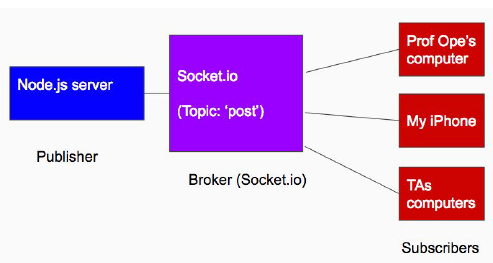
\includegraphics[width=0.4\textwidth]{./pub-sub1}
    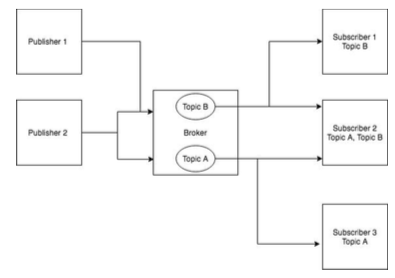
\includegraphics[width=0.4\textwidth]{./pub-sub2}
\end{center}

\pattern{Pipe and Filter}
\begin{summary}

    A very simple, powerful, and robust architectural style comprised of
    filters, which are used to transform data, and pipes, which pass the data
    between them.

    {\bf Pipe and filter} is most useful for asynchronous systems with many
    data transformations and large processes that can be broken down into
    sub-tasks. The style allows concurrent and modular application of filters
    to subsets of the data. Filters must sometimes be serialized (applied
    one after another) and thus don’t always benefit from concurrency (but
    still benefit from modularity). 
    
    This architectural style also applies to systems where the output of one
    program becomes the input of another program like the UNIX pipe command
    (which is where the name comes from).

\end{summary}

\subsubsection{Implementation}

\begin{description}
    \item[Pipe] Carries and transfers data between components (pumps,
        filters, and sinks). Pipes are directional streams of data, and are
        generally implemented as a type of data buffer which stores data until
        the next filter or sink is available to take the data and process it. A
        pipe can be thought of as a connector between two components.

    \item[Filter] A component of the system which performs some processing to
        the data delivered to it by a pipe. The processed data is output to
        another pipe. A filter can have any amount of input and output pipes.

    \item[Pump] A data source to the overall system. Pumps can be files as well
        as input devices such as keyboards, mice, etc.

    \item[Sink] The ultimate data target (output receiver) of the system.
        Sinks can be files, databases, output devices (screen, speakers), etc.
\end{description}

\comparison{\begin{description}
        \item[Modularity] Components can be pipelined together in many
            different combinations to create novel applications. Each component
            is completely separate for maintenance and development purposes.

        \item[Scalability] Developers can compile and run components in
            parallel since they have defined inputs and outputs with no side
            effects.

        \item[Maintainability] Components do not rely on the implementation of
            each other, so are easy to test. The encapsulation is useful to
            create hierarchy and simplifies the use of this style.

        \item[Maintainabilty] The style creates reusable code due to the
            separation of concerns of each component

    \end{description}
}{\begin{description}
        \item[Flexibility] Pipe-and-filter is not ideal for passing complex
            data structures between the components, because they would need to
            be serialized to a common data type. 

            It is not useful when components need to interact because pipes do
            not allow shared access. If the filters are distributed, the
            usual caveats of distributed computing apply.

    \end{description}
}% END Comparison

\begin{nfps}
\item[Efficiency] Filters work independently to each other, which leads to a
    very efficient workflow as no components depend on others to work.

\item[Scalability] The system can be scaled up or down by simply adding or
    removing filters and different pipes.

\item[Maintainability] As mentioned previously. 
    
\item[Negative Evolvability] The cost and development time of the design might
    be higher than similar designs, as each component is designed individually. 

\item [Negative Resilience] Since one broken filter can defect the entire
    system, if it is the only instance, and the work cannot be rescheduled.

\end{nfps}

\begin{center}
    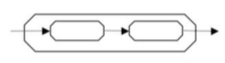
\includegraphics[width=0.4\textwidth]{./pipe-filter}
    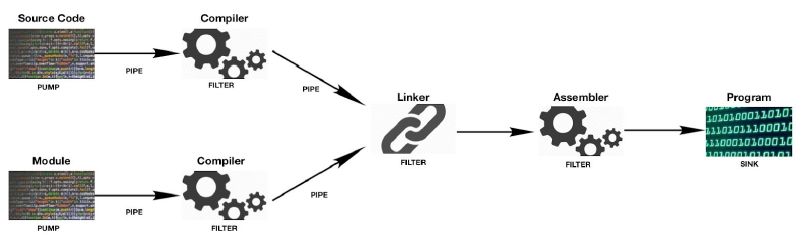
\includegraphics[width=0.4\textwidth]{./pipe-filter2}
\end{center}

\pattern{Peer to Peer (P2P)}
\begin{summary}
Computers (called peers) communicate directly with one another, instead of
through a centralized server

Data is transferred without a central server (a central server may be used to
connect peers, either built into the protocol or as an external service that
users use to find each other)

Each peer acts as both a client and a server, meaning each peer can make
requests for data and respond to requests for data

Only requirement is an internet connection and a P2P application, and peers
using the same protocol

Inherently connected to file sharing, P2P network requests usually represent a
file request.
\end{summary}

\comparison{\begin{itemize}
        \item Scalability: P2P architecture is particularly useful for
            distributing large files. This architecture is able to solve 
            the problem of bandwidth and network scaling which exists in other
            architectures. Namely, that there are too many requests and data
            through too few internet ``pipes''. If connections to main google
            data centres fail, large parts of internet go down. 

        \item Scalability: It is expensive to route data through high-bandwidth
            cable instead of low-bandwidth cable, more connections is less
            expensive. 

        \item Scalability: P2P limits data speed to only the cable going into
            your house, instead of to the slowest cable in the route to a
            server.
\end{itemize}
}{\begin{itemize}
        \item Performance/availability: Peer-to-peer systems may not be able to
            consistently achieve the same performance and availability. Throughput
            is reliant on the existence of seeders. Popular files are easily
            and highly distributed, but unpopular files eventually disappear
            and become unavailable as people stop sharing them. Additionally,
            performance highly dependent on selection of right peers at right
            time.
        \item Administration: There is usually no centralized administrative
            control over the system. However, managing security, data
            consistency, data/service availability, backup, and recovery are
            the responsibility of the end users or their applications. 
        \item Security \& trust: Vulnerabilities in systems can be easily
            distributed/taken advantage of, for example: corrupted data and
            malware spreads very quickly. Additionally, each IP is publicly
            available to all peers in the network.
    \end{itemize}
}% END comparison

\begin{nfps}
\item[Efficiency] With server-client, the server must send copies of files
    sequentially and each client must download a file from the server, often
    using one connection. In contrast, with peer-to-peer the files are shared
    between peers, removing load from the server. Decrease in bandwidth cost
    for the distributors, the bandwidth is distributed among peers.

\item[Scalability] In server-client, distribution time increases linearly with
    number of users; in P2P, in increases logarithmically with number of users. 

\item[Dependability] P2P networks are fault tolerant: there is no dependency on
    a single, central server (except perhaps for the optional tracker server). 
    Capacity of the network increases as peers arrive, and the failure of a
    peer does not mean failure of the network. Additionally, no government or
    corporation can stop P2P file sharing without blocking all internet access.
    The resilience of network increases as number of peers increases. 

\item[Maintainability] No need to maintain the network in most situations.

\item[Negative Evolvability] Software using this architecture is inherently
    distributed, therefore any changes to the design would require each
    individual nodes P2P application to be updated and for the users to update
    their applications independently. However, P2P networks function
    independent of end-user software
\end{nfps}

\begin{center}
    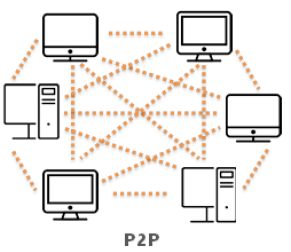
\includegraphics[width=0.4\textwidth]{./peer-to-peer}
\end{center}

\pattern{Mobile Code}
\begin{summary}
an application that is capable of movement while embedded in internet services
such as web pages and emails. The components are made of two parts:
Compiler/Interpreter and Execution Dock. The compiler/interpreter is
responsible for interpreting the code received. The execution dock is
responsible for receiving and executing the code. The components are connected
via network, mainly HTTP. Using the established network, data such as program
code or program state are transferred.

There are three variants to the architecture: Code-on-demand, Remote execution,
and Mobile agents. Code-on-demand variant moves code from a server to clients,
utilizing clients’ resources to execute the code. The remote execution works
the opposite, by sending a code from a client to a server. The client in this
case can utilize the process power of the server, if resources are limited
locally. Lastly, mobile agents allow communication between clients. A mobile
code can move from one client to another to add more resources to run the code.
\end{summary}

\comparison{\begin{itemize}
        \item Highly dynamically adaptable: the application can seamlessly be
started on any mobile platform (client) without actually changing the code.
This is a very critical non-functional property; without the ability to be
dynamic, the mobile code architecture loses its’ identity. By keeping the
underlying structure of the code the same across all mobile platforms, no
modifications are needed to be made to the code.

\item remote usability: this is also another non-functional
property. This aspect of the architecture allows the code to be quickly
evaluated or executed on any mobile device in the system. It is supported by
the network connectivity and underlying framework. This means that any of the
clients have the ability to compile code, or push it to another device for
compilation. 

\item efficient resource utilization. With mobile
code architecture, one device can autonomously migrate to or employ a different
node in the system in order to obtain more resources. Overall, these features
lead to better performance. Typically, data can run faster when it is closer to
its parent dataset. In these cases, the program would experience a higher
throughput because it takes less time for each packet of data to transfer.

\end{itemize}
}{\begin{itemize}
        \item dependability: While network connectivity serves as a powerful
            resource to the mobile code architecture, it serves as a major
            point of failure. This architecture relies entirely on a solid
            network connection. If this connection were to degrade, the system
            would be rendered useless. 

        \item efficency:  Another drawback is the increased amounts of data
            being transmitted. A repository of code that has not yet been
            compiled is a significant order of magnitude greater in size than
            the compiled version.  Initially, there would be a lot more data
            transmitted using this architecture as opposed to just transmitting
            the results yielded by the application.  Additionally, transmitting
            all of this code takes more time. 

        \item dependability A huge flaw in this architecture is that it allows major
            security breaches. Transmitting the code base for an application over a
            network of devices leaves a huge amount of room for hackers and malicious
            attacks. This is also known as the underlying architecture for a variety of
            destructive programs such as worms, trojans, rogues, and malware.
    \end{itemize}
} %END comparison

\begin{nfps}
\item[Low Coupling] While different variations of the Mobile Code architecture
    may result in varying degrees of coupling between components, the use of
    this style typically results in reductions in coupling, especially when
    developers rely on open standards which are well established. Using the
    Code on Demand variant, clients are interchangeable from the perspective of
    the servers which they interact with, since all of the clients (mobile
    devices) have web browsers which conform to the same standards regardless
    of maker. Similarly, the Remote Execution pattern allows for low coupling
    between mobile devices and servers, as long as the code which they desire
    to execute remotely conforms to the interpreter which runs on the server.
    Both of these variants result in lower coupling than their alternatives.
    Finally however, the Mobile Agent relies on a bit more coupling, as mobile
    devices must rely on each other as well as servers for resource sharing,
    meaning that there’s increased complexity in ensuring various types of
    mobile devices are interoperable. This results in moderate coupling between
    the modules which must run on these different devices.
\end{nfps}

\begin{center}
    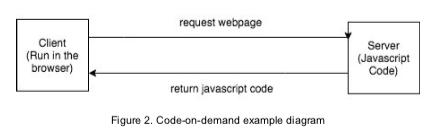
\includegraphics[width=0.4\textwidth]{./mobile-code1}
    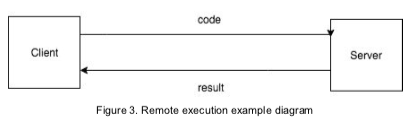
\includegraphics[width=0.4\textwidth]{./mobile-code2}
    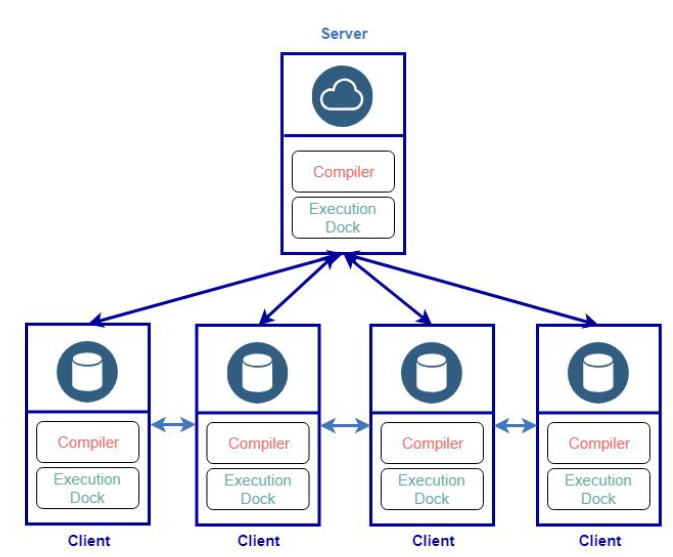
\includegraphics[width=0.4\textwidth]{./mobile-code3}
\end{center}

\pattern{Layered}
\begin{summary}
    A layered architecture style divides components into layers with specific
    functions. For each unique project, there is no specified number of layers
    that it must possess and developers decide on the number of layers
    depending on the needs of the project. This architecture is best suited for
    microservices, and systems without much business logic to complicate
    relationships between layers.  This is because each layer is only required
    to fulfill its own responsibilities without taking on the responsibilities
    of the other layers for the sake of organization. Over the years, it has
    become the most popular style due to its simplicity, ease of development,
    and organization.  
\end{summary}

\comparison{\begin{itemize}
        \item Testability: Components can be mocked or stubbed since they
            belong to specific layers of the architecture. Due to this, it is
            relatively easy to test functionality of isolated functionalities.
            For example, a presentation component can be mocked to focus on
            testing a business component, or the business layer can be mocked
            to test certain aspects of the presentation layer.

        \item Maintainability: Layers are created to separate the concerns of
            the components. As an example, business logic should only be
            contained in the business layer. Because of this, if there are
            changes to one layer, other layers’ components should not be
            affected, making layers easy to update and maintain for future
            changes.

        \item Ease of development for teams: Since this pattern is very well
            known and simple to understand, it also provides teams with ease of
            development. Different people are usually given tasks specific to
            their domain of knowledge, so it makes sense for each person to
            focus on their tasks without having to understand all parts of the
            application. As an example, a person who works on the presentation
            layer does not need to know how data is stored in the database
            layer. Likewise, a person that works on the database layer does not
            need to understand how the presentation layer is implemented. Thus
            the architecture supports the non-functional requirement of
            complexity.

        \item Cohesion: If each layer is well defined and only contains
            functions that are related to the needs of that layer, the layer
            has high cohesion. For example, the database layer should only have
            components which deal with writing, querying, and generally
            managing the data.

        \item Coupling: Each layer is considered to be either open or closed.
            Requests can bypass open layers, while if the layer is closed the
            request must go through that layer. There should be clear
            documentation or communication of which are open and closed, and
            the reason for their implementation. Depending on their
            architecture, layers can provide low coupling. However, a layered
            architecture can have high coupling, which is a disadvantage, if
            software developers or architects do not follow best practices.

\end{itemize}
}{\begin{itemize}
        \item Low Scalability: Due to the nature of layered architecture being
            very simple, it is difficult to use its principles on larger and
            more complex projects. This is due to the architecture being
            monolithic in nature, and further organization and complexity is
            difficult to implement without abstracting from the layered
            principle. For example, it is possible to further abstract each
            layer adding complexity but it is difficult to keep the simple
            layered architecture principles. Therefore, since the architecture
            offers little support and guidelines for expanding to meet the
            requirements of larger and more complex projects the non functional
            property of scalability is low.

        \item Inefficiencies: As perceived from the diagrams thus far, a
            potential request may have to go through multiple layers to fulfill
            a request. Although this can be somewhat alleviated with open and
            closed layers, the architecture as a whole suffers from general
            inefficiency as requests need to often go through multiple layers
            instead of one source. Difficult to Deploy: In cases where layers
            or components (a common pitfall using the architecture
            historically) within the layer are highly coupled, it creates a
            scenario where layers or components highly depend on each other.
            Then, it becomes that changing one component needs several other
            components to be affected and thus rebuilt, which takes time. Thus,
            it is often not efficient for highly coupled layers to be used in
            things like a continuous deployment pipeline.
            
        \item Low Agility: Also due to the potential coupling, the pattern
            itself may have low agility which is a non functional property
            which measures how the architecture responds to quick continuous
            changes. Although some features can be isolated in this pattern, if
            components or layers are highly coupled, changing a component may
            cause the developer to need to make changes in other components and
            layers if they depend on each other. Since coupling between
            components within layers is a common pitfall using this
            architecture, it generally does not meet the non functional
            property of agility.
\end{itemize}}

\begin{nfps}
\item[Description] See above.
\end{nfps}

\begin{center}
    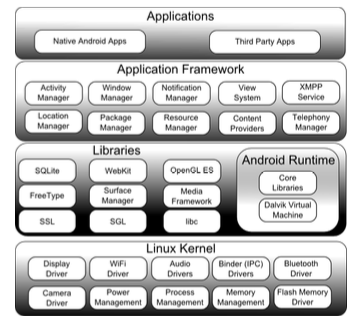
\includegraphics[width=0.4\textwidth]{./layered}
    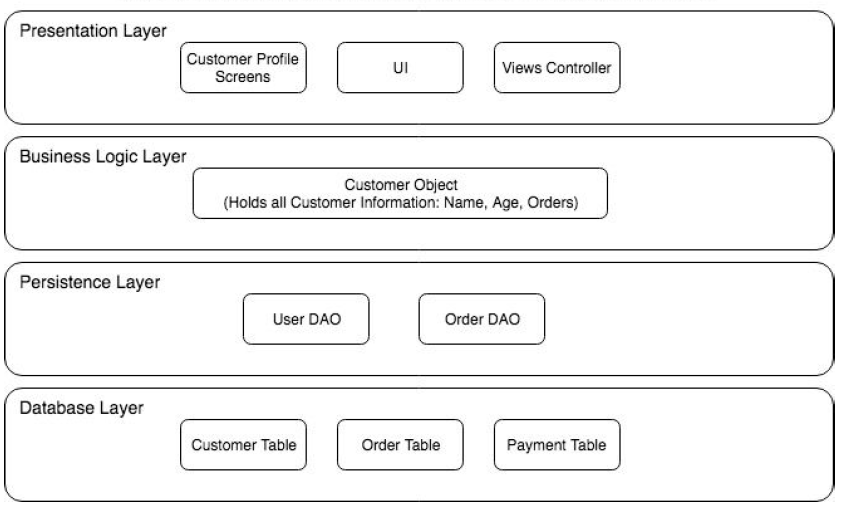
\includegraphics[width=0.4\textwidth]{./layered2}
\end{center}

\pattern{Interpreter}

\begin{summary}
    An interpreter is a computer program that directly executes , i.e.
    performs, instructions written in a programming or scripting language ,
    without requiring them previously to have been compiled into a machine
    language program.  Interpreters translate the (source) code instructions
    one by one and execute them. For example, Python.

    The interpreter style is an architectural style that is suitable for
    applications in which the most appropriate language or machine for
    executing the solution is not directly available.

    Interpreter style is also called virtual machine style. The virtual machine
    often includes the pseudo code that is to be interpreted and the
    interpreter engine.

    The interpreter engine includes the syntax interpreter and the current
    state of the interpreter. To pass data from one instruction to the other we
    need to keep the interpreter state. The interpreter parses and executes
    input commands and then updates the state maintained by the interpreter. We
    usually use a data structure that records the current state of the
    interpreter.

    There are procedure calls used for communication between interpreter engine
    and the pseudo code. And also, direct memory access is involved when
    reading and storing data of the source code, state of the source code and
    the state of interpreter.
\end{summary}

\subsubsection{Implementation}
There are four components in the interpreter architecture:
1. interpreter. 
2. current state of the interpreter. 
3. program being interpreted. 
4. current state of the program being interpreted.

There are two connectors for interpreter architecture:
1. Procedure calls. 
2. Direct memory accesses.

\comparison{\begin{itemize}
        \item Interpreters can be used to run scripts and macros. A macro
            records keyboard and mouse inputs so that they can be executed
            later. This allows users to record interactions with the user
            interface which may be either repetitive or complex, and then
            replay the recorded actions in a simple and quick way.

        \item An interpreter allows you to add functionality to a system, or
            extend existing functionality of a system. This is done by
            composing pre-existing functions together in a specific sequence,
            and in order to create something new. These pre-existing functions
            are defined by the system architecture and offered to the user. The
            developer, thus, avoids the need to implement all possible
            combinations of functionality.

        \item Having a system with a built in interpreter is not only
            beneficial to developers, it encourages end users to implement
            their own customizations. Toward this end, a system can offer an
            easier way to use language that has domain specific abstractions
            suited to the needs and thinking of the end users.

        \item 1. Interpreters encourage end users to implement their own
            customizations. This is an advance over requiring end users to use
            the general programming languages that professional software
            developers use.

        \item 2. Easy for debugging. It will examine each line and the results
            of the execution are visible. Errors are caught as they happen
            since the interpreter stops when it can’t interpret a line. This is
            very helpful for people to debug.

        \item 3. Less memory. Compare to executable file. Because only a few
            lines of source code needs to be in memory at any one time.

        \item 4. This can make your system more portable, it can work on
            platforms that the interpreter supports.
\end{itemize}
}{\begin{itemize}
        \item Performance: Basic implementation spend little time analyzing the
            source code and use a line by line translate and execute strategy.
            This is a classic trade off, it may be faster and more flexible for
            developers to use the interpretive language, but slower for the
            computer to execute it.
\end{itemize}}

\begin{nfps}
\item[Programmability] An interpreter allows users to add functionality to the
    system or extend existing functionality of a system. For example, a web
    browser extension which is different from a plug in, is a component that
    adds new functionality to the browsers. These extensions can be written in
    different languages depending on the browsers. It is run by an interpreter
    which is embedded in the browser. For example in firefox, it can be written
    in C++ or Javascript. Therefore, it offers an easier way for developers to
    customize their own functionalities.

\item[Portability and flexibility] As virtual machines and virtual
    environments increasing, portability is becoming more and more important.
    In compiler, the binary code produced by compiler is tailored specifically
    to a target computer architecture. But in reality, web applications must
    run in different kinds of machines, so it not effective for the browser to
    download the binary representation of the remote software. However,
    interpreter can process the source code directly so that it can allow those
    machine code intended for one hardware architecture to be run on another
    using a virtual machine. This can greatly facilitate the portability and
    flexibility of applications or languages across various platforms.

\item[Security] An interpreter or virtual machine does not execute all the
    source code blindly. Instead it can refuse to execute code that violates
    any security constraints. A typical example is JS-Interpreter which can
    sandbox potentially hostile code. This kind of interpreter is secure by
    creating its own virtual machine. External APIs is not acceptable unless
    provided by the developers. Therefore, it can protect the system from
    potential hostile code.

\end{nfps}

\begin{center}
    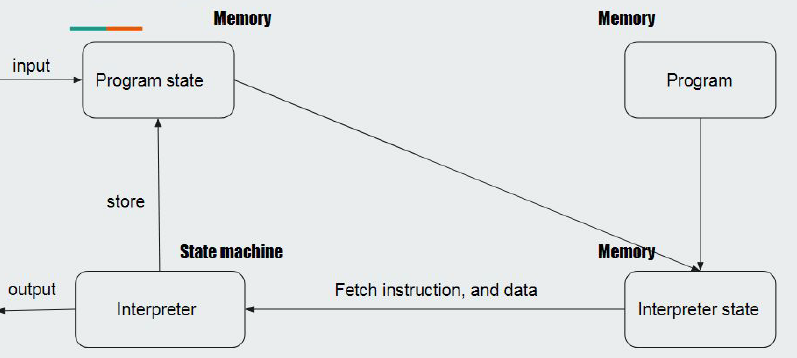
\includegraphics[width=0.4\textwidth]{./interpreter}
\end{center}

\pattern{Event Based}
\begin{summary}
Event-based architecture is an architecture style that uses the production and
consumption of events to control the behaviour of components. Instead of
components communicate directly by referencing or method call, they communicate
by sending and receiving events asynchronously.

There are two types of components call event producer and event consumer. Event
producer is a component that produces and sends event. It should maintain its
internal state and produce an event when some predefined state change happened.
Event  consumer is a component that receives and consumers event. It should
consumer the event that it receives and starts its process with respect to the
event. One component can be both event producer and consumer interchangeably in
the context of entire architecture by both producing and consuming events.
There is only one type of connector in this architecture called event bus.
Event bus is the medium on which the events are being transmitted.

Event-based architectures can simplify software design, development, and
testing because they minimize the connections between the components. Instead
of each component directly communicate to each other with high coupling and
complicated structure, they all communicate through the event bus which makes
communication elegant. Each component can be developed and tested independently
because they do not require to know other components. This can be very
beneficial to large projects since the complexity of the project grows linearly
instead of exponential.

Most applicable to specific kinds of problems \begin{itemize}[noitemsep]
    \item User interface: website browser
    \item Distributed application
\end{itemize}

\end{summary}

\comparison{\begin{itemize}
        \item Engender specific kinds of change resilience: 
● For removing an event bus and creating producers before creating an event
bus, we need to change producers to handle the invalid event bus because
producers might not be able to fire an event to an empty place/address
● For changing an event type for a typed event bus, we also need to maintain
consistency for producers and consumers as well. 
\end{itemize}
}{\begin{itemize}
        \item The event bus may become a bottleneck.
○ When there are too many producers are sending the message concurrently.
Therefore, the number of messages is larger than the number of events which the
event bus handled.
● Not sending message efficiency.
○ The event bus has the queue for event sending or receive. It can not send or
receive the message immediately. 
\end{itemize}}

\begin{nfps}
\item[Scalability] The Space decoupling
■ The event producers and event consumers do not need to know each other.
■ The event producers do not hold references to event consumers or know how many of them are interacting and vice versa.
○ The time decoupling
■ The event producers and event consumers do not need to be actively involved in the interaction at the same time.
○ The synchronization decoupling
■ The event producers are not blocked while producing events and they can receive events.
■ The event consumers can get the notification when an event happens while performing some other concurrent activity.
● Easy to evolve
○ The architecture is loose coupling, you can easily create a new event to the event bus.
● Great distribution
○ The event can be almost anything and exists almost anywhere.
2. Scalability: As shown above, we can separate customer by adding priority. Then, delete the previous customer component, add high priority and low priority components. So, the event bus will handle requests according to priority.

\item[Testability] each component can be tested by itself since their input and
    output is testable.
\end{nfps}

\begin{center}
    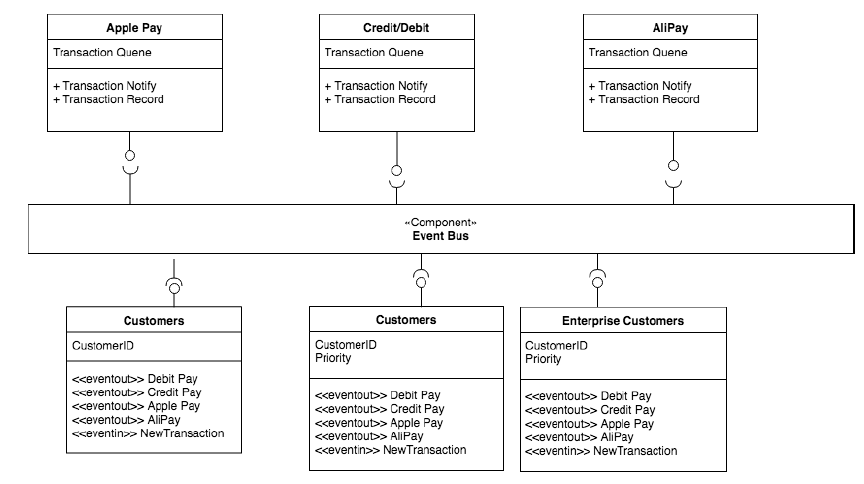
\includegraphics[width=0.4\textwidth]{./event-based}
\end{center}

\pattern{Distributed}
\begin{summary}
Distributed objects is a combination and adaptation of many simpler
architectures. It is derived from object-oriented and client-server
architecture which allows for objects to be distributed and accessed. When
developing applications using this architecture, it is very easy to come across
some constraints such as cross-machine and cross-language communication. To
address this, additional styles are applied such as pipe-filtering which allow
for serialization of parameters which creates uniform communication. This
process of filtering, serializing parameters is known as data marshaling.
\end{summary}

\comparison{\begin{itemize}
        \item Engender change resilience: The increased redundancy in a
            distributed system can increase its resiliency. Hardware is prone
            to failure, so by distributing the functionality and data across a
            cluster of machines, this allows the system to recover from
            unforeseen crashes. When certain machines are down, the system can
            still retain its full functionality since the remaining nodes in
            the cluster are able to pick up the slack by doing its work. For
            this to work, the data is also stored redundantly amongst the
            cluster to ensure that a copy of the data is always available even
            when a portion of the cluster is offline. By the nature of its
            design, distributed objects also makes the system more scalable.
            When there is a big increase in demand, the cluster manager can
            spin up more machines in the cluster during runtime to accommodate
            for the extra requests. The performance and resiliency of a cluster
            can be changed without altering its functionality, this is done by
            changing the size of the cluster.
\end{itemize}
}{\begin{itemize}
        \item Using distributed objects allows systems to be designed and
            developed using segments that are written in different languages
            with different platforms. However, this induces the applications to
            be built in the distributed objects style. The first negative
            behaviour is exhibited in the interactions of components, it tends
            to be mostly synchronous and it does not take the advantage of
            distributed systems concurrency. In terms of object interactions,
            many distributed object style applications may have trouble dealing
            with data traversal in streams, and also having difficulties with
            asynchronous invocations. This induces the distributed objects
            style on the application building process without regarding if it’s
            the best style for the application.

        \item In terms of the components in a distributed objects style,
            they are required to explicitly specify the provided interfaces,
            however, it does not specifying required interfaces, which may
            cause deeply ingrained dependencies between objects. Another
            negative behaviour exhibiting from distributed objects style is
            that the objects are created, linked, and destroyed constantly. Due
            to all the creation and destruction of the objects, it’s difficult
            to fully comprehend the structure and configurations of the
            application at any given time.
\end{itemize}}

\begin{nfps}
\item[None] Gonna have to dig in the rest of this text for them.
\end{nfps}

\subsubsection{Implementation}

Implementation of Distributed Objects may involve several important
aspects. Firstly, a class named “Matrix Class” is initialized in a generic,
broad object language. That matrix class actually defines the inner components
and functions like methods. Most of the times, such is IDL: Interface
Description Language.
At the very initial stage of compilation, the matrix class is changed to every
listed languages, whether they be C++, Java, etc. Every program subsequently
involves the feasible file in their system. These blocks of codes comprise of
the definition of classes as well as methods for disintegrating the actual
class to several components. This transmits them via a connection to other
program, regenerating the object on the opposite side.

\begin{center}
    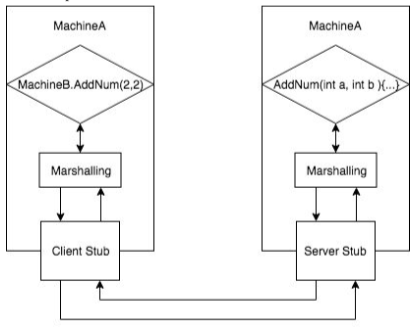
\includegraphics[width=0.48\textwidth]{./distributed1}
    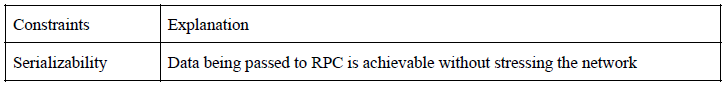
\includegraphics[width=0.48\textwidth]{./distributed2}
    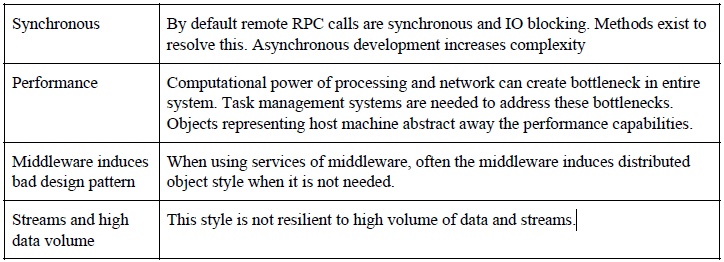
\includegraphics[width=0.48\textwidth]{./distributed3}
    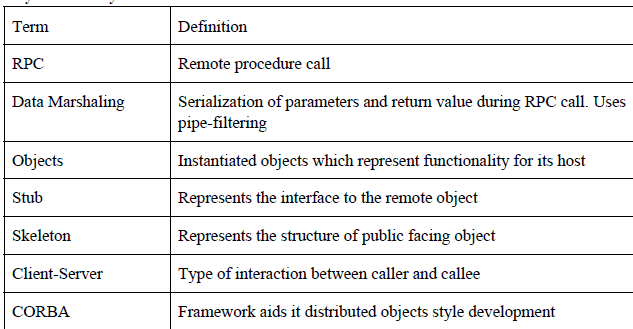
\includegraphics[width=0.48\textwidth]{./distributed4}
\end{center}

\pattern{Client Server}
\begin{summary}
    The client-server architecture is a pure network architecture in which each
    computer or process on the network is either a client or a server. There
    are 3 major components. First we have the servers which are powerful
    computers or processes dedicated to managing disk drives (file servers),
    printers (print servers), or network traffic (network servers). Second,
    clients are workstations on which users can run applications. Finally we
    have resources which are files, devices, and even processing power. The
    components are connected via connectors which are essentially network layer
    protocols such as TCP/IP.
\end{summary}

\comparison{\begin{itemize}

        \item The architecture style allows the system to distribute workload
            amongst multiple machines or processes. It is very flexible as to
            allow the architect to decide how to divide tasks amongst the
            clients and servers. This helps promote the separation of concerns.
            The architecture style is most beneficial when increasing the
            modularity of the components and decreasing coupling. This can be
            done through encapsulation of information with a well-defined
            standardized interface. The system will also allow centralized
            control and redesign since all machines and processes should be
            running software defined by the system architect.

\end{itemize}
}{\begin{itemize}
        \item Due to its centralized design, need load-balancer and failover
            systems in order to scale properly. There is a possibility for
            congestion of traffic, which motivates the need for the
            load-balancers. A client-server network is also costly to set up,
            often requiring you to purchase licenses like a copy of Windows NT,
            which is a family of operating systems for servers, and also client
            licenses. The hardware required for servers is also needed to be
            more powerful than a standard workstation, and additionally require
            employees to manage them. This means paying more for equipment and
            networking professionals, who don’t come cheap, to even run the
            server.

        \item The client-server system is especially vulnerable to failures as
            there is always going to be a limited number of servers relative to
            clients. If a critical number of them go down, no users will be
            able to use the system until the servers are fixed or replaced.
            This makes them vulnerable to denial of service attack, distributed
            denial of service attack where the perpetrator seeks to make a
            machine or network resource unavailable to its intended users by
            temporarily or indefinitely disrupting services of a host connected
            to the Internet. Denial of service is typically accomplished by
            flooding the targeted machine or resource with superfluous requests
            in an attempt to overload systems
\end{itemize}}

\begin{nfps}
\item[Dependability] The architecture supports availability as servers are easy
    to keep running and typically do not have to shutdown or restart for many
    days. It also supports dependability as control and distribution of
    resources and data are controlled by a dedicated server. 
\item[Heterogeneity] clients and servers often function as disparate parts. 
\item[Scalability] the centralized servers can be updated with minimal impact
    to the client.

\item[Negative Efficiency] since the server handles all the stress and demand
    of the system. When there is an unanticipated amount of stress and the
    server becomes congested, performance can slow down drastically or even
    fail to perform which affects all users. 
\item[Negative Transparency?] It also inhibits transparency because
    communication is restricted to requests and clients are unable to see fetch
    processes running on the server.
\end{nfps}

\subsubsection{Implementation and Example}

As seen from the diagrams, the flow of the data is unidirectional and forms a
cycle. It is usually initiated by the client requesting some kind of data and
the server processing the request and sending some kind of data back to the
client. A typical topological data flow goes as follows:
\begin{enumerate}[noitemsep]
    \item Client request data from server
    \item Load balancer routes the request to the appropriate server
    \item Server process the request client
    \item Server queries appropriate database for some data
    \item Database return the queried data back the server
    \item The server processes the data and send the data back to the client
    \item (This process repeats)
\end{enumerate}

All technology companies today use this architecture, Uber, Facebook, Airbnb,
etc.
\begin{center}
    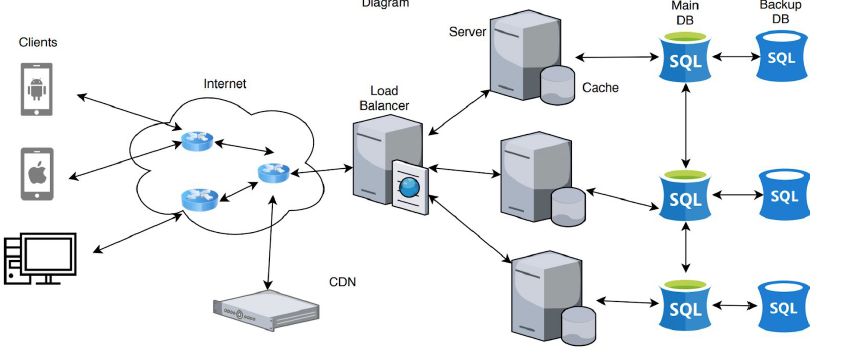
\includegraphics[width=0.4\textwidth]{./client-server}
\end{center}

\pattern{Blackboard}
\begin{summary}
a behavioural design pattern for systems that need to integrate multiple
individually specialized computation modules to solve complex problems where
information is ambiguous, and the path to the solution is not known in advance.
Its architectural topology can be separated into 3 main sub-categories: the
blackboard, the knowledge sources, and the controller, as shown in Figure 1. In
general, the blackboard is a shared memory space holding information
representing the state of a problem on which knowledge sources (KS) will
operate when recruited by the controller, applying their specialized knowledge
to contribute to the ultimate formation of a solution. This cooperative process
will be discussed in more detail in the next sections.

The blackboard architecture is ideal for solving problems where information is
ambiguous or the path to the solution is not known in advance. The blackboard
is a shared memory space that is responsible for acting as a hub for all
streamed data, solutions, and partial solutions. The KSs, also called “experts”
or “agents”, are responsible for performing very specific tasks to contribute
to the final solution. A KS is generally used to determine if the problem has
been solved or solved enough. Not all KSs need to contribute to a solution or
to be run in order to sufficiently find the solution to a problem. Controllers
are used to orchestrate the KSs. Many algorithms can be used with the
controller to help optimize the execution of KSs.

The blackboard is a shared memory space. This means that all the information
streamed into the system or processed by the KSs will persist in this shared
space, fully accessible by all components in the system. At any given point in
time, the blackboard is not required to have the full solution to the problem
the system is built for. Instead, it will hold partial solutions to smaller
subproblems solved and, eventually, due to the non-deterministic nature of the
control process, will contain a solution that is deemed viable to a certain
degree of precision. The KSs are the “experts” responsible for processing and
contributing to the solution as a whole.

\end{summary}

\subsubsection{Implementation}

Knowledge sources, also called agents, can be thought of as specialised
“experts” in being able to perform very specific tasks. From the perspective of
the blackboard, the KSs form a panel of individuals, unaware of each other, who
will contribute their niche resources to advance the problem toward an
acceptable solution state. Incidentally, this decoupling of resources makes
blackboard architecture very modular, making reuse of KSs very easy for new
blackboard implementations. Collectively, the incremental solutions processed
and reposted to the blackboard by the KSs will converge on a solution. One of
the KSs may be responsible for marking a solution presented on the blackboard
as “viable”. The degree of the viability of a solution depends entirely on the
problem and the defined criteria for an acceptable solution.

In some implementations of this architecture, a controller is not even
necessary. The KSs evaluate the information presented on the blackboard and, if
able, they process them on their own, possibly editing metadata associated with
the information they want to process to keep track of the problem state.
However, the purpose of this pattern is to provide an architectural framework
that is capable of solving complex, non-deterministic control problems. This
means that the KSs may not necessarily run linearly; they can run in parallel.
Optimization is at the root of control problems where resource allocation in
parallel computation is necessary to most efficiently compute a solution to a
problem. This is where a controller comes into the picture to help address the
optimization problem.

The controller is responsible for assigning tasks to the KSs to process
information on the blackboard. The goal is to converge on a solution that is
considered acceptable for the problem. The way in which the controller,
blackboard, and KSs communicate (i.e. event-based, polling,
publisher-subscriber, etc.) is less important than the roles they play, and
thus not rigidly defined in the architecture.

% \comparison{\begin{itemize}

% \end{itemize}
% }{\begin{itemize}

% \end{itemize}}

\begin{nfps}
\item[Reusable] A single KS can be used by multiple blackboards. Since they are independent from each other, they can be reused in other blackboard architecture problems.

\item[Scalable] Because of the flexibility of the KSs it is easy to add and
    remove them. If we wish to have a better solution, adding agents could
    help. The controller just needs to be modified to take into consideration
    the changes. Overall, if the system requires more processing power, then
    additional agents can be added to create a better throughput.

\item[Robust] If a KS fails to complete its task or is unavailable, then a
    solution might still be found thanks to the other KSs. Note that it might
    not be as optimal or complete.

\end{nfps}

\begin{center}
    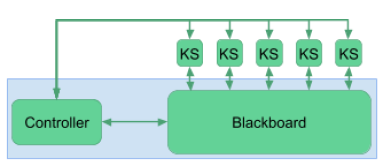
\includegraphics[width=0.4\textwidth]{./blackboard}
\end{center}


\end{document}
